\chapter{Learning Optimal Decision Sets and Lists with SAT}\label{chap:jair21}


This chapter is based on:
\begin{itemize}
	\item Jinqiang Yu, Alexey Ignatiev, Peter J. Stuckey, and Pierre Le Bodic. Learning optimal decision
sets and lists with sat. \emph{Journal of Artificial Intelligence Research,} 72, 1251-1279, 2021.
\end{itemize}

The most interpretable ML models include decision sets and decision lists,
since these models consist of straightforward logical rules.
%
Decision sets offer the simplest explanation because when a rule that ``fires'' for a given data
point, that rule alone suffices as the explanation, 
while for decision lists, i.e. ordered sets of rules, we have to also
consider the order of rules in the model.
%
To ensure these models are easily understandable to humans, 
their succinctness should be maximized.
%
A recent study has proposed an method to compute decision sets, focusing initially on minimizing the number of 
rules and afterwards minimizing the number of literals.
%
Additionally, there has been investigation~\cite{meel-cp18,meel-aies19}
into developing a CNF classifier 
that minimizes the number of literals within a fixed number of rules,
aimed at generating interpretable decision rules to explain instances of the positive class.
%
However, we argue that previous studies have not used the most best explainability measure.
%
For example, two rules, each consisting of 80 conditions, are notably less interpretable
than four rules, each comprising only 10 conditions.
%
Motivated by this, we explore directly computing decision sets and lists 
that minimize their size, redefined as the total number of literals in the model.
%
This lead to smaller decision sets and decision lists~(in terms of literals),
which are considered more appealing for explaining decisions.
%
This chapter introduces methods for learning ``perfect'' decision sets and decision lists with
minimum size, which are perfectly accurate on the training data, with the use of SAT solving technology.
%
Furthermore, this chapter presents a novel approach to identifying optimal sparse alternatives, 
trading of accuracy and size.


%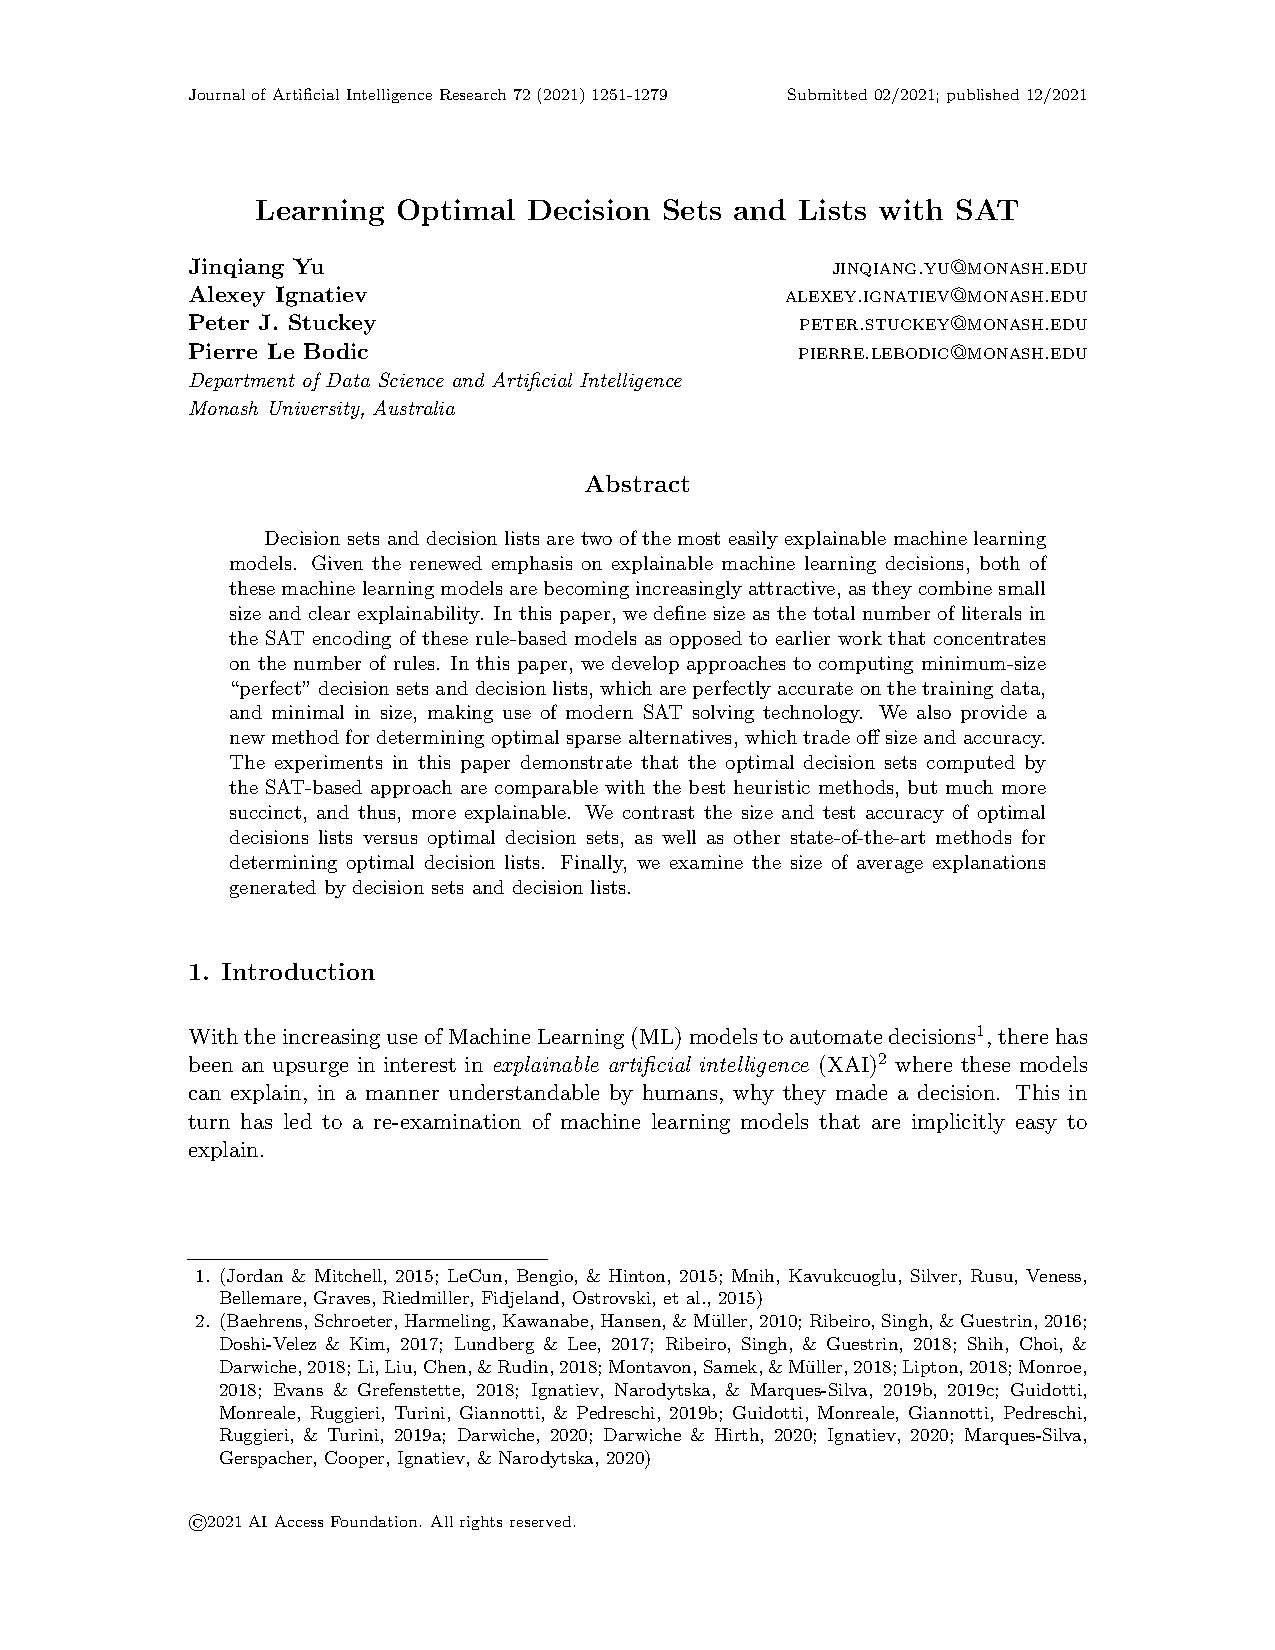
\includepdf[pages=-, offset=75 -75]{papers/jair21.pdf}
